%%%%%%%%%%%%%%%%%%%%%%%%%%%%%%%%%%%%%%%%%
\documentclass[paper=a4, fontsize=15pt]{article} % A4 paper and 11pt font size

\usepackage{amsmath,amsfonts,amsthm} % Math packages
\usepackage{graphicx}
\usepackage[top=0.5in, bottom=1in, left=1in, right=1in]{geometry}
\usepackage{tabularx}


\pagestyle{plain} % Makes all pages in the document conform to the custom headers and footers

\title{	
Machine Learning \\
Homework 3
}
\author{Yao Song\\301266041} % Your name
\date{\normalsize\today} % Today's date or a custom date

\begin{document}
\maketitle % Print the title
%----------------------------------------------------------------------------------------
%	PROBLEM 1
%----------------------------------------------------------------------------------------

\section*{Question 1}
\begin{align}
&\frac{\mathrm d}{\mathrm d x} \left( (1+\exp(-a)^{-1}) \right) \\
=&-(1+\exp(-a))^{-2} \frac{\mathrm d}{\mathrm d x} \left( \exp(-a) \right)\\
=& \frac{exp(-a)}{(1+\exp(-a))^{2}}\\
=& \frac{1}{1+\exp(-a)} - \frac{1}{(1+\exp(-a))^{2}}\\
=& g(a) - g(a)^2\\
=& g(a)( 1- g(a) )
\end{align}

%%%%%%%%%%%%%%%%%%%%%%%%%%%%%%%%%%%%%%%%%%%%%%%%%%%%%%%%%%%%%%%%%%%%%%%%%%%%%%%%%%

\section*{Question 2}
\subsection*{1}
No. They are not independent.
\subsection*{2}
The assumption is reasonable. Because the driver's age is not necessarily reflected on the mileage of the vehicle. It may be a second hand car owned by a new driver or an experienced driver may just get a new car.
\subsection*{3}
The ExtraCar node tells us something about the SocioEcon, which will affect the MedicalCost.
So ExtraCar information is useful in determining MedicalCost in an indirect way.
For example, if we know a customer has an extra car, his or her SocioEcon is more likely to be better than the customer's SocioEcon without an extra car. So we know this customer is able to afford more insurance cost. That is important information to be incorporated into our determination.
\subsection*{4}
Denote MeicalCost = x,  LiabilityCost = y,  PropertyCost =z, age= a, VehicleYear = v. 
Then the expectation of the total insurance cost of the prospective client can be written as follows:
\begin{align}
E[x+y+z|a,v]
& = \int_x \int_y \int_z (x+y+z) Pr(x,y,z|a,v)\, dxdydz,   \nonumber
\end{align}
where $Pr(x,y,z|a,v)$ is the joint conditional probability of $x,y,z$ given $a$ and $v$.




%%%%%%%%%%%%%%%%%%%%%%%%%%%%%%%%%%%%%%%%%%%%%%%%%%%%%%%%%%%%%%%%%%%%%%%%%%%%%%%%%%
\section*{Question 3}
The likelihood function can be written as 
\begin{align}
L(\boldsymbol{\theta})
& = P(\textbf{x}^1,\textbf{x}^1,\ldots,\textbf{x}^N | \boldsymbol{\theta})\\
& = \prod_{i=1}^N P(\textbf{x}^i | \boldsymbol{\theta})
  =  \prod_{i=1}^N P({x}^i_1,{x}^i_2,\ldots,{x}^i_D | \boldsymbol{\theta})\\
& = \prod_{i=1}^N \prod_{k=1}^D P(x_k^i | pa_k; \boldsymbol{\theta}_k)\\
& = \prod_{k=1}^D P(x_k^1,x_k^2,\ldots,x_k^N | pa_k; \boldsymbol{\theta}_k)\\
& = \prod_{k=1}^D P(\boldsymbol{x_k} | pa_k; \boldsymbol{\theta}_k)
\end{align}
where we have defined $\boldsymbol{x_k}  = [x_k^1,x_k^2,\ldots,x_k^N]$. So we can see that learning the parameters for the network according to the maximum likelihood criterion can be done by separately learning the parameters $\boldsymbol{\theta}_k$ of each conditional distribution using the relevant components of the training data.
%%%%%%%%%%%%%%%%%%%%%%%%%%%%%%%%%%%%%%%%%%%%%%%%%%%%%%%%%%%%%%%%%%%%%%%%%%%%%%%%%%



\section*{Question 4}
\subsection*{1}
Please see the plot in the last page.
\begin{figure}[hb]
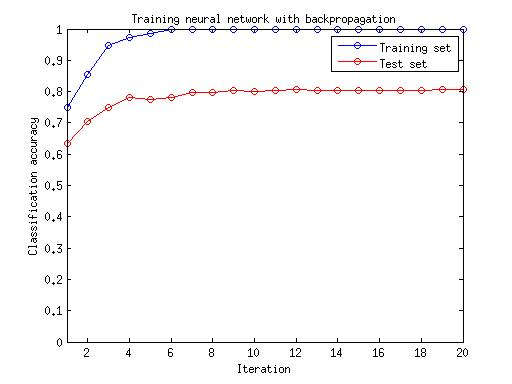
\includegraphics[width=\linewidth]{./a3_datacode/normal.jpg}
\caption{training/testing error plot}
\label{fig:normal}
\end{figure}

\subsection*{2}
By commenting out line 39 in the code, I changed the initialization of the first layer weights.
\subsection*{3}
The first thing we can observe is the accuracy does not change any more.
Going one step further, we will find dW1 and dW2 do not change.
So the weights will not change. Obviously that is due to the improper initialization of the weights.
When we go into the process, we can observe that the returned values $A$ and $Z$ from the function "feedforward" do not change at all. So we need to analyze the feedfoward function.

By analysis of feedfoward function, we can find that $A_{1}$ has large values. That makes $Z_{1} =1./(1+exp(-A_{1}))$ equal to vector of ones and remain unchanged. 

If we add line39 in the code. We can observe $A_{1}$ with small values and as a result $Z_{1}$ will have different values and keep changing.
%%%%%%%%%%%%%%%%%%%%%%%%%%%%%%%%%%%%%%%%%%%%%%%%%%%%%%%%%%%%%%%%%%%%%%%%%%%%%%%%%%




%----------------------------------------------------------------------------------------

\end{document}